
\subsection{Running TUG Wizard}

This section describes how to deploy TUG Wizard. Please, follow the steps
described in the following.

%\setcounter{enumi}{4}
\begin{enumerate}
%
%%% 
%%
\item {\bf Step 1: Unpack TUG package.}\\
%
  {\tt TUG Wizard} as well as
  {\tt TUGLib} are packed into a file named {\tt
    TUG\_vXX.tar.gz}. \\Unpack this package into a folder. As a result
  you will get a set of files as depicted in the figure below.

\vspace{1ex}
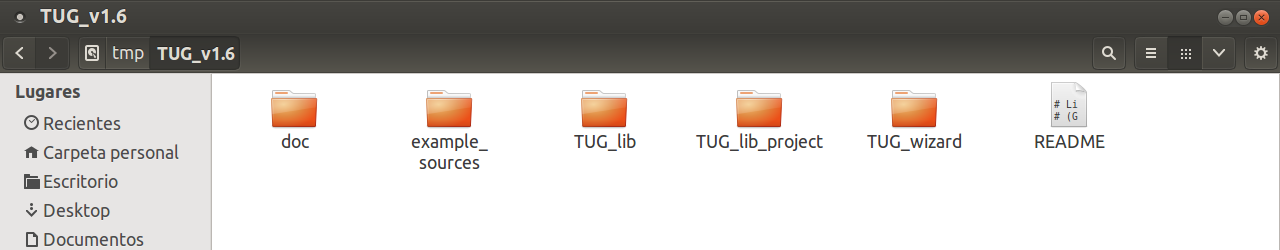
\includegraphics[width=.95\textwidth]{images/tug011.png}
\vspace{3ex}
%
%%% 
%%
\item {\bf Step 2: Launch TUG Wizard.}\\
%
  Go to {\tt TUG\_Wizard}
  folder. \\Add execution permission to the script file {\tt
    launch\_TUGWizard} as depicted in the figure below. \\Execute 
  {\tt launch\_TUGWizard} to launch the wizard prompt. 

\vspace{1ex}
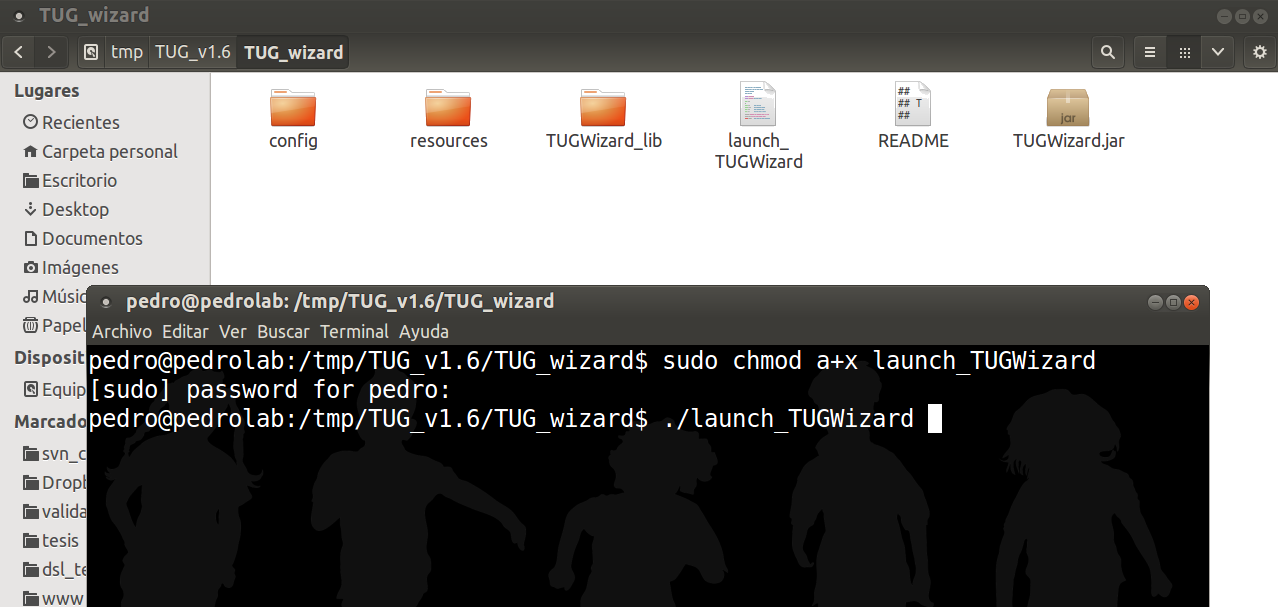
\includegraphics[width=.95\textwidth]{images/tug012.png}
\vspace{3ex}
\newpage
%
%%% 
%%
\item {\bf Step 3: TUG Wizard ready.}\\
%
  After the execution of the two
  steps described above, TUG Wizard will be prompted to start the
  configuration and generation of a testing project, as described in
  next section.

\vspace{1ex}
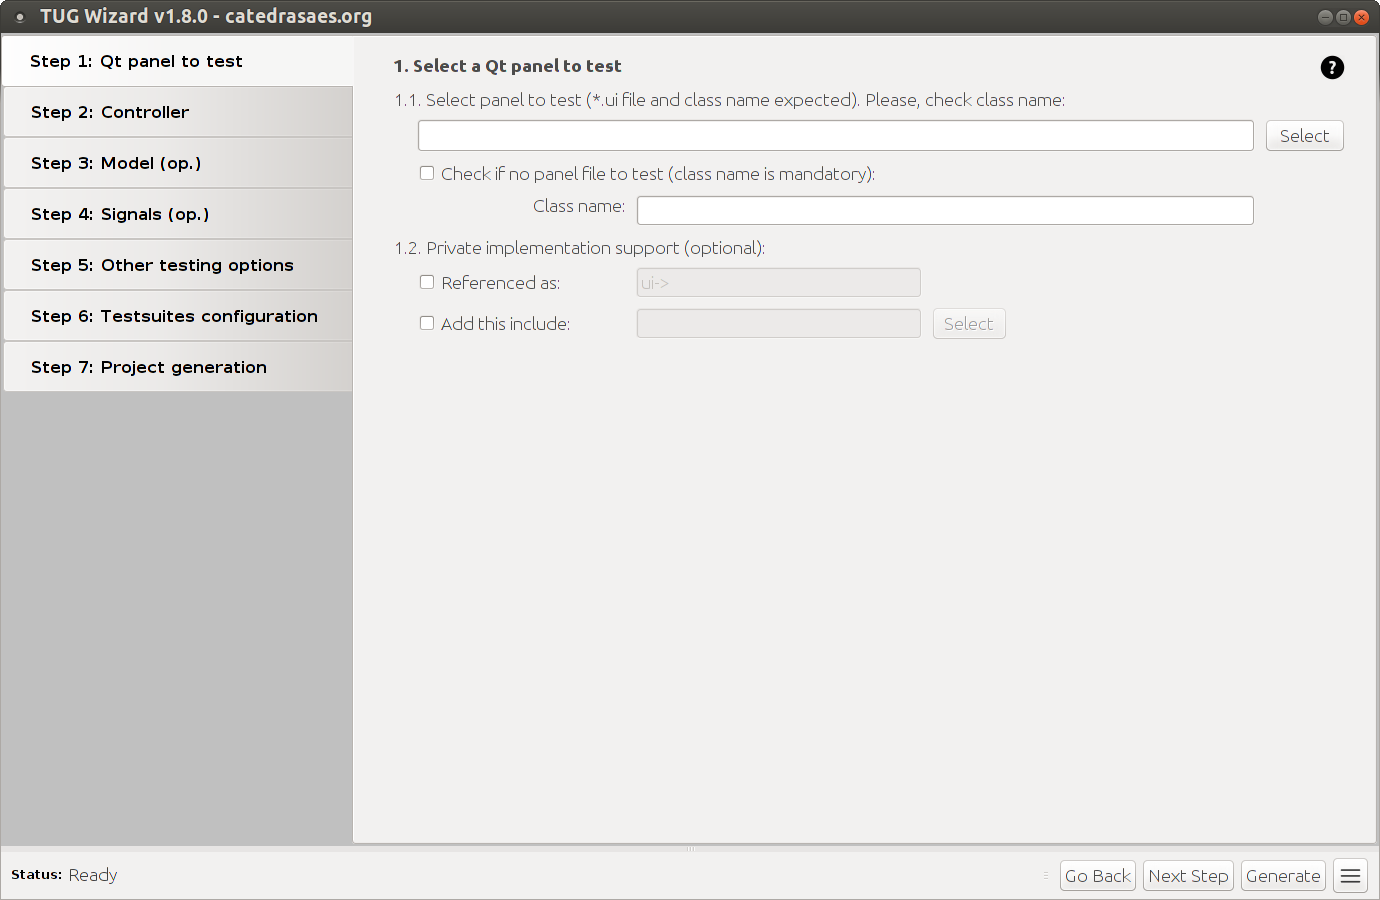
\includegraphics[width=.95\textwidth]{images/tug013.png}
\vspace{3ex}
\end{enumerate}
\newpage




%%% Local variables:
%%% mode: latex
%%% TeX-master: "README.tex"
%%% ispell-local-dictionary: "american"
%%% coding: utf-8
%%% fill-column: 75
%%% TeX-parse-self: t
%%% TeX-auto-save: t
%%% End:
